\begin{figure*}[ht]
\begin{center}
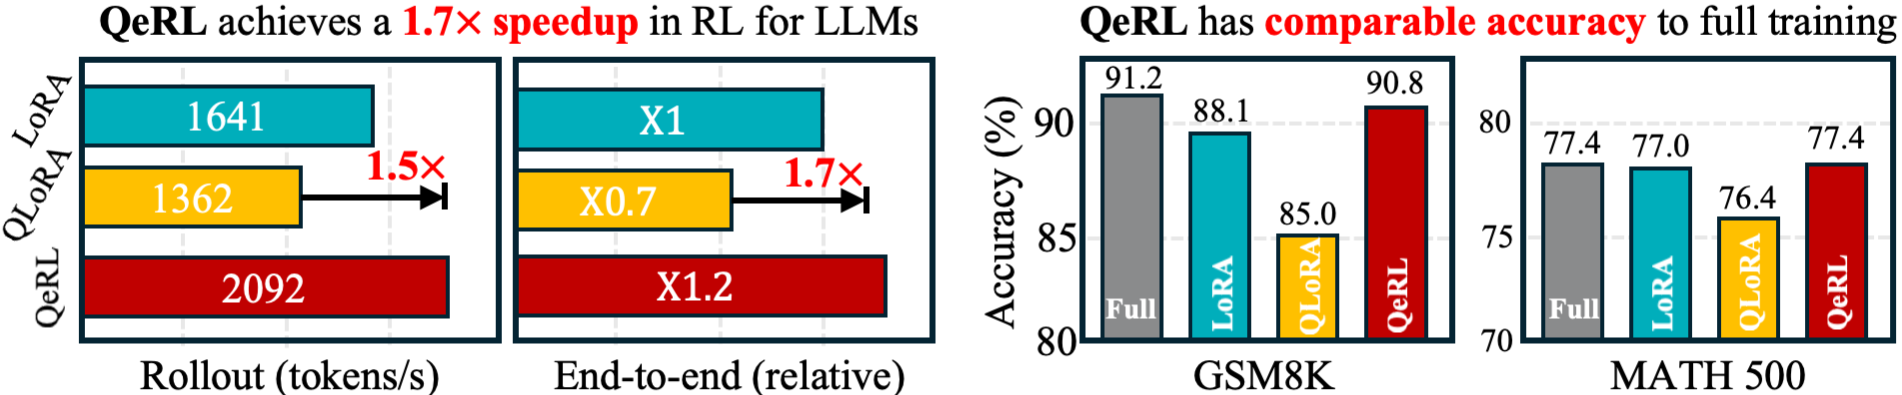
\includegraphics[width=\linewidth]{figures/performance.png}
\end{center}
\vspace{-0.1in}
\caption{Rollout speedup and accuracy of \QeRL $\,$ on Qwen2.5-7B-Instruct. \QeRL $\,$ achieves faster RL rollout and end-to-end training speeds (batch=8), while delivering performance superior to vanilla LoRA and QLoRA, also comparable to full-parameter RL on mathematical benchmarks.}
\vspace{-0.1in}
\label{fig:performance}
\end{figure*}

\section{Introduction}
% large language model reasoning important, RL 对于 reasoning 重要
% The ability to perform multi-step reasoning is essential for large language models (LLMs) to tackle complex tasks, ranging from theoretical problem-solving to practical decision-making~\citep{survey-efficient-reasoning,survey-reinforced-reasoning,sft-rl-study}. Supervised fine-tuning (SFT) is a widely adopted approach to enhance reasoning, often training models to replicate explicit reasoning traces, such as step-by-step demonstrations~\citep{o1-replication,slow-thinking}. While effective, this approach risks encouraging superficial imitation rather than fostering genuine exploration of reasoning pathways. In contrast, reinforcement learning (RL) leverages verifiable reward signals to promote adaptive learning, allowing models to explore diverse logical trajectories and discover more robust solutions~\citep{tulu-3}. By optimizing behavior through interaction and feedback, RL enables models to generalize more effectively to large-scale or open-ended reasoning tasks compared to pure imitation learning~\citep{deepseek-r1}.
The ability to perform multi-step reasoning is critical for large language models (LLMs) to handle complex tasks, from theoretical problem solving to practical decision making~\citep{survey-efficient-reasoning, survey-reinforced-reasoning, sft-rl-study,yang2021multiple}. Supervised fine-tuning (SFT) is a common method to improve reasoning by training models to replicate explicit reasoning steps~\citep{o1-replication, slow-thinking}. However, this approach risks promoting imitation rather than encouraging genuine reasoning. In contrast, reinforcement learning (RL) uses verifiable reward signals to support adaptive learning, allowing models to explore diverse reasoning traces and identify more robust solutions~\citep{tulu-3,deepseek-r1,chen2025scaling}. 

% RL 训练代价大，model size 大
% Despite its advantages, RL training for reasoning in LLMs is highly resource-intensive and complex. In terms of memory, RL pipelines often require significant GPU resources, as multiple models (e.g., policy and reference models in GRPO~\citep{grpo}) must be maintained simultaneously. Additionally, reasoning-focused LLMs are typically very large~\citep{deepseek-r1}, further compounding memory demands. In terms of training speed, RL involves multi-stage processes—such as rollouts, reward computation, logit evaluation, and gradient updates—that significantly slow down training. Rollouts, in particular, are computationally expensive, requiring repeated sampling; for complex reasoning tasks, each rollout can involve processing extremely long sequences (e.g., tens of thousands of tokens in mathematical benchmarks)~\citep{dapo}. Furthermore, RL is notoriously sample-inefficient~\citep{sample-efficiency}, which exacerbates training time and computational costs.
RL is effective for LLMs' reasoning but highly resource-intensive. RL requires substantial GPU memory, as multiple models, such as policy and reference models in GRPO~\citep{grpo}, must run concurrently. The large size of reasoning-focused LLMs~\citep{deepseek-r1} further exacerbates memory demands. Training is also slowed by multistage processes, including rollouts, reward computation, logit evaluation, and gradient updates. Rollouts are particularly costly, involving repeated sampling and processing of long sequences for complex tasks~\citep{dapo}. Additionally, RL’s inherent sample inefficiency~\citep{sample-efficiency} further increases costs.

\begin{figure*}[t]
\begin{center}
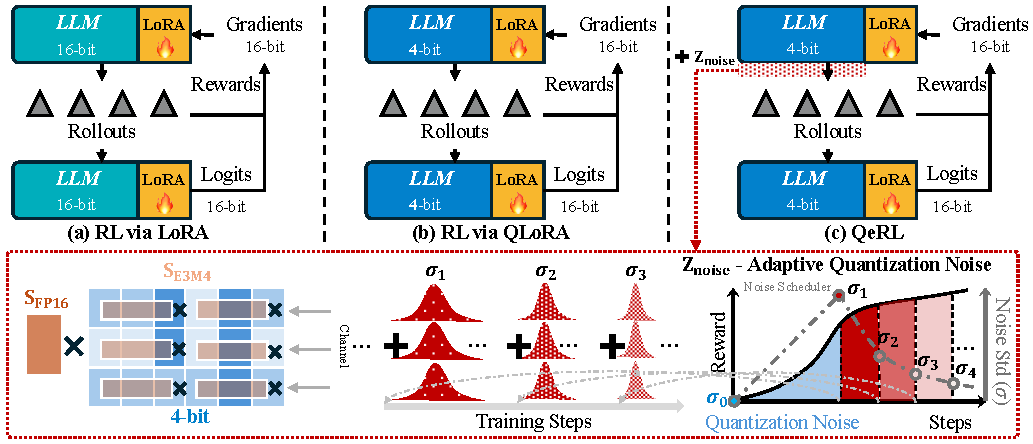
\includegraphics[width=\linewidth]{figures/framework4.pdf}
\end{center}
\vspace{-0.1in}
\caption{The illustration of \QeRL. (a) \textbf{RL via LoRA}: reducing trainable parameters, but does not alleviate the rollout bottleneck. (b) \textbf{RL via QLoRA}: NF4 quantization with LoRA, but NF4 is slower than LoRA. (c) \textbf{\QeRL}: NVFP4 quantization with LoRA, reducing memory and enabling faster RL while matching full-parameter finetuning performance with adaptive quantization noise. AQN dynamically adjusts quantization noise with an exponential scheduler, enhancing exploration.}
\vspace{-0.1in}
\label{fig:framework}
\end{figure*}

% Existing efficient RL methods, (1) quantized rollout (Flash-RL) - update 开销大、16 bit 和 8 bit 两个models, memory 大, (2) LoRA (Tina: Tiny Reasoning Models via LoRA), memory 大
% While various methods have been proposed to improve the efficiency of RL in LLMs, they still face notable limitations. The first category of approaches, such as Tina~\citep{tina}, adopts parameter-efficient fine-tuning techniques like Low-Rank Adaptation (LoRA)~\citep{lora} to reduce the number of trainable parameters. However, similar to the use of LoRA in SFT\citep{longlora}, these methods fail to address the fundamental bottleneck of slow rollout speeds. The second category, represented by FlashRL~\citep{liu2025flashrl}, relies on quantized rollout models to reduce computational costs. However, due to the precision mismatch between the rollout model and the logits model (e.g., 8-bit vs. 16-bit), importance sampling is required to correct discrepancies between the two models. This necessitates maintaining both 8-bit and 16-bit models simultaneously, resulting in increased memory overhead. Additionally, directly applying QLoRA~\citep{qlora} with NormalFloat 4-bit (NF4) precision introduces higher computation costs, increasing rollout time by 1.5 to 2 times, further limiting its efficiency.
Improving RL efficiency in LLMs presents significant challenges. One approach, exemplified by Tina~\citep{tina}, leverages parameter-efficient fine-tuning methods like Low-Rank Adaptation (LoRA)~\citep{lora} to reduce trainable parameters. However, similar to LoRA in SFT~\citep{longlora}, these methods fail to address the core issue of slow rollout speeds. Another strategy, demonstrated by FlashRL~\citep{liu2025flashrl}, uses quantized rollout models to reduce computational costs. However, precision mismatches between the rollout model and logits model (e.g., 8-bit vs. 16-bit) require importance sampling to correct discrepancies, necessitating both 8-bit and 16-bit models to run simultaneously, which increases memory usage. To overcome these limitations, we focus on lower-bit quantization while avoiding duplicate models in memory. Additionally, using QLoRA~\citep{qlora} in RL slows rollouts by 1.5–2$\times$, further reducing efficiency. This slowdown occurs because QLoRA relies on NormalFloat 4-bit (NF4) precision, which requires unpacking and mapping to floating-point values via a lookup table before matrix multiplication.
%\xjqi{add a statement of NF4. Despite of significantly reducing memory costs, ...... can split and move to next paragraph}

% （Our methods+finding）我们惊讶的发现quantization 模型能够帮助exploration。。。。。。（提一嘴我们用lora方式training）。highlight 4bit+lora在reward上升速度和最终accuracy优于16bit+lora。特别是在最新的NVFP4数据格式下。
% 我们提出了一种deformable quantization noise 。。。。。。dynamic，可变噪声。。。。
% In this paper, we propose \QeRL, a {{Quantization}}-enhanced {{Reinforcement Learning}} framework for LLMs.
% Beyond efficiency, quantization improves exploration during RL training.
% As shown in Fig.~\ref{fig:framework}, we incorporate LoRA layers to enable gradient back-propagation through quantized weights. 
% Surprisingly, our empirical results show that quantization not only improves training efficiency but also strengthens policy exploration during RL training, as shown in Fig.~\ref{fig:entropy_abs}. 
% Motivated by this finding, we introduce a deformable quantization noise strategy that dynamically adjusts the degree of exploration across training steps. 
% With 4-bit LLMs, \QeRL $\,$ achieves faster reward growth and higher final accuracy compared to 16-bit LoRA baselines, and even comparable to full-parameter training, as shown in Fig.~\ref{fig:performance}.
% Our empirical study revealed an intriguing finding: quantized LLMs not only reduce memory overhead during training but also achieve higher reward improvements in RL compared to their 16-bit counterparts. This result contrasts with conclusions drawn from vanilla SFT of LLMs~\citep{qlora,guo2023lq}. As shown in Fig.~\ref{fig:entropy_abs}, we observed that quantization noise, introduced by quantization errors, increases the policy entropy of the model, thereby enhancing uncertainty during exploration. This boost in entropy facilitates the discovery of better strategies in RL~\citep{cui2025entropy}, similar to the role of parameter noise in traditional RL techniques~\citeauthor{plappert2017parameter}. However, directly applying QLoRA~\citep{qlora} to reinforcement learning (RL) presents two major challenges: \textbf{1)} The NF4 precision format significantly increases inference latency, leading to higher computational costs during rollouts and reduced training efficiency; \textbf{2)} The deterministic nature of quantization noise lacks the adaptability of stochastic noise sampling, which is crucial for dynamically enhancing policy exploration in RL. While quantization noise can facilitate exploration, the large errors introduced by NF4 can negatively impact the subsequent stages of training.

% To address these challenges, we propose \textbf{QeRL}, a quantization-based RL framework tailored for training LLMs on reasoning tasks. As illustrated in Fig.~\ref{fig:framework}, \textbf{QeRL} employs NVFP4 quantization for LLM weights while integrating a Triton-based~\citep{noauthor_tritonpythontritonopsmatmulpy_nodate} high-performance inference kernel. This design accelerates rollout and prefilling speeds without compromising accuracy, with gradient backpropagation enabled through LoRA layers. To mitigate the limitations of static quantization noise, we introduce an \textbf{adaptive quantization noise (AQN)} mechanism that injects channel-wise random noise during RL training. AQN dynamically adjusts exploration noise as training progresses, following a geometric decay schedule. Furthermore, we adopt a noise-sharing technique that merges the noise vector into the layer normalization layer, enabling zero-parameter overhead noise injection. Compared to the vanilla LoRA baseline, QeRL achieves faster RL training speeds, enhanced reward growth, and higher final accuracy. For instance, as shown in Fig.\ref{fig:performance}, QeRL outperforms QLoRA and vanilla LoRA in rollout and prefilling speed on the Qwen2.5-7B-Instruct model. It achieves a GSM8K score of 90.8, surpassing both 16-bit LoRA and QLoRA, and matches the accuracy of full-parameter fine-tuning on MATH 500. Extensive experiments demonstrate that QeRL consistently outperforms 16-bit LoRA across models of various sizes in terms of memory efficiency, training speed, and reward performance, while closely matching the performance of full-parameter fine-tuning.

% Standard quantization methods worsen this limitation as they are stochastic and lack precise noise control. is static and deterministic, lacking the adaptive variability required for effective exploration.

To address the limitations of NF4 in QLoRA, a natural solution is to adopt higher-performance quantization.
However, standard quantization methods introduce static and deterministic noise, which is non-beneficial to the later-stage RL training.
To avoid this drawback, our analysis surprisingly reveals that quantization noise, with precise control, can benefit RL by increasing policy entropy (Fig.\ref{fig:entropy_abs}). This added entropy enhances exploration by introducing uncertainty, similar to the effect of parameter noise in RL~\citep{plappert2017parameter,pang2021robust}, and helps models discover better strategies~\citep{cui2025entropy}. 
Our experiments show that a well-designed noise strategy allows quantized LLMs to exploit this effect, reducing memory overhead while gaining better reward curves. This finding contrasts with results from SFT of LLMs~\citep{qlora, guo2023lq}, demonstrating that controllable quantization noise in RL enhances exploration and enables quantized frameworks to surpass 16-bit LoRA in both efficiency and performance.

%Although this finding might contrast with prior conclusions drawn from vanilla SFT of LLMs~\citep{qlora, guo2023lq}. 
%\xjqi{The transition here is a bit strange, better to connect with previous paragraphs to show why you do this study} 
%
%\xjqi{Despite of this, the deterministic nature of quantization ......}
%However, applying QLoRA~\citep{qlora} directly to RL presents two key challenges: \textbf{1)} The NF4 precision format significantly increases inference latency, raising computational costs during rollouts and reducing training efficiency; 
%While quantization noise can aid exploration, the large errors introduced by NF4 can negatively affect subsequent training stages.
%\xjqi{which stages ?? so you also reduce the quantization error?}

% To address these challenges, we propose \textbf{QeRL}, a quantization-based RL framework tailored for training LLMs on reasoning tasks. As illustrated in Fig.\ref{fig:framework}, \textbf{QeRL} employs NVFP4 quantization for LLM weights and integrates a Marlin-based~\citep{frantar2024marlin} in both rollout and prefilling stages. This design accelerates rollout and prefilling speeds without compromising accuracy, with gradient backpropagation supported through LoRA layers. To overcome the limitations of static quantization noise, we introduce an \textbf{adaptive quantization noise (AQN)} mechanism that injects channel-wise random noise during training, dynamically adjusting exploration noise using a geometric decay schedule. Additionally, we implement a noise-sharing technique that merges the noise vector into the layer normalization layer, enabling zero-parameter overhead noise injection. Compared to the vanilla LoRA baseline, QeRL achieves faster training, improved reward growth, and higher accuracy. For instance, as shown in Fig.~\ref{fig:performance}, QeRL outperforms QLoRA and vanilla LoRA in rollout and prefilling speeds on the Qwen2.5-7B-Instruct model, achieving a GSM8K score of 90.8, which surpasses both 16-bit LoRA and QLoRA, while matching the accuracy of full-parameter fine-tuning on MATH 500. Experiments show QeRL outperforms vanilla LoRA and QLoRA in memory efficiency, training speed, and rewards performance, while matching full fine-tuning. QeRL can even trains a 32B model with GRPO on a single H100 80GB GPU.

We propose QeRL, a quantization-based RL framework designed to train LLMs on reasoning tasks. As shown in Fig.\ref{fig:framework}, QeRL uses NVFP4 quantization for LLM weights and integrates a Marlin-based~\citep{frantar2024marlin} approach in both rollout and prefilling stages. This design accelerates rollout and prefilling without sacrificing accuracy, with gradient backpropagation enabled through LoRA layers. To address static quantization noise, we introduce adaptive quantization noise (AQN), which injects channel-wise random noise during training and adjusts exploration noise dynamically using an exponential schedule. Additionally, we implement a noise-sharing strategy that merges the noise vector into the layer normalization layer, enabling zero-parameter overhead for noise injection. Compared to vanilla LoRA, QeRL achieves faster rollout and better reward growth. For example, as shown in Fig.\ref{fig:performance}, QeRL outperforms QLoRA and vanilla LoRA in rollout and prefilling speeds on the Qwen2.5-7B-Instruct model, achieving a GSM8K score of 90.8—surpassing both 16-bit LoRA and QLoRA while matching full fine-tuning accuracy on MATH 500. QeRL outperforms vanilla LoRA and QLoRA in both training speed and reward performance. Notably, it achieves approximately a 1.8$\times$ speedup in end-to-end training, compared to QLoRA. Additionally, QeRL demonstrates the capability to train a 32B model with GRPO on a single H100 80GB GPU.

\begin{figure*}[t]
\begin{center}
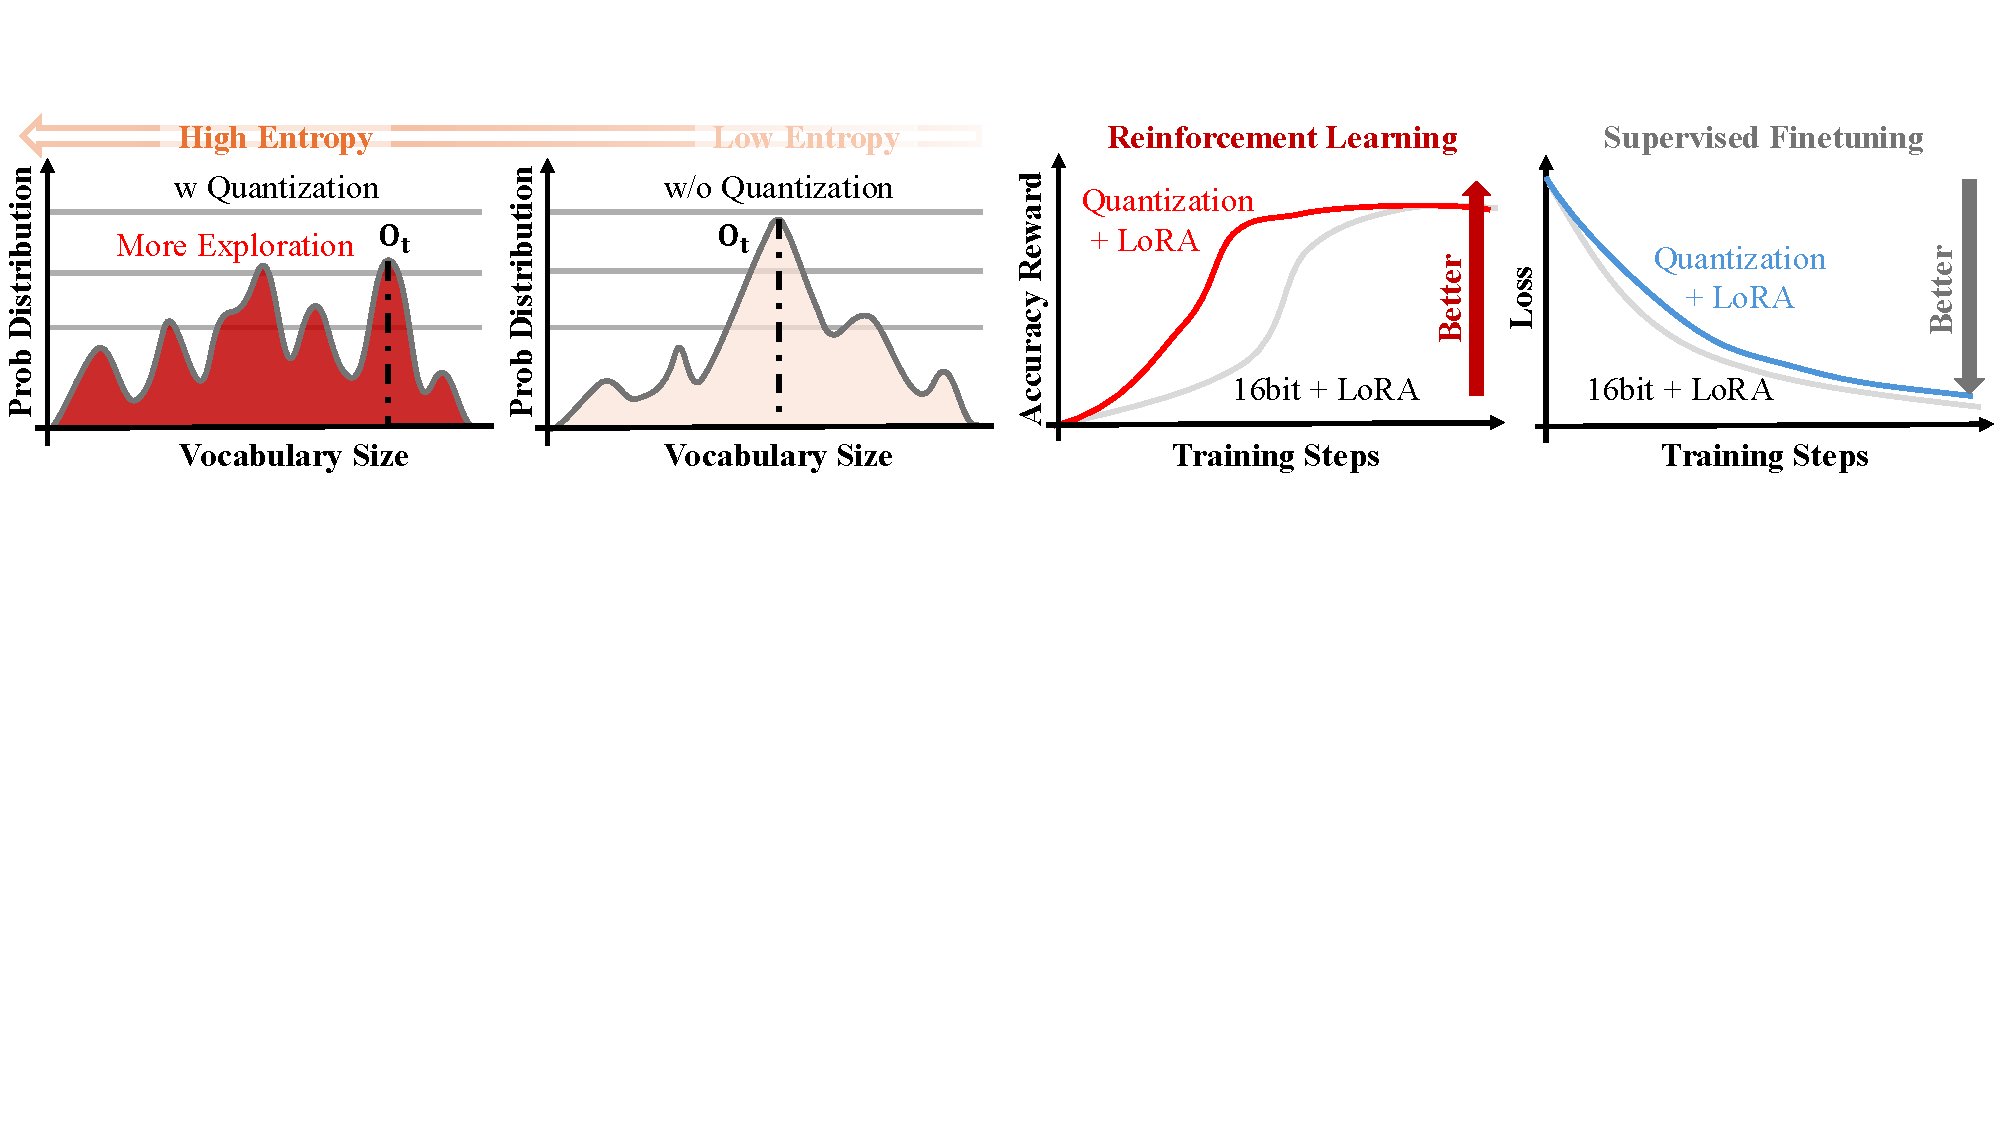
\includegraphics[width=\linewidth]{figures/entropy_abs_line_v2.pdf}
\end{center}
\vspace{-0.1in}
\caption{Advancement of Quantization in RL Exploration. Quantization noise brings higher initialized entropy, which encourages exploration in RL training, accelerating the increase of reward. }
\label{fig:entropy_abs}
\vspace{-0.1in}
\end{figure*}

% Experiments